\chapter{The Hall Effects}

\label{chapter2}

\section{Introduction - Ordinary Hall effect}

These effects originally deal with the application of an external magnetic field on a current carrying material and subsequently observing the effect either on the conductor or the electric current itself.

In 1879, Edwin Hall was exploring this interaction and tried to determine the effect of the magnetic field on a current carrying wire, with a suspicion that it either affected the whole length of the wire or only the moving electrons.

He later devised a rather simple experiment based on the argument that ``if the current of electricity in a fixed conductor is itself attracted by a magnet, the current should be drawn to one side of the wire, and therefore the resistance experienced should be increased." \autocite[1]{S.1880}

Hall couldn't detect this extra resistance (which we now know as magnetoresistance) but concluded that a transverse force in the opposite direction must exist and which appears as a transverse voltage across the width of the conducting material. This is the Hall effect and the transverse voltage is the Hall voltage.

The experiment by Hall is shown in the figure below.

\begin{figure}[h] \label{hall-figure} 
    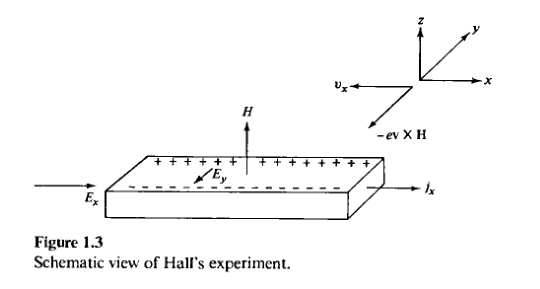
\includegraphics[width=0.7\columnwidth]{hall-effect-ashcroft.png}
    \caption{Schematic diagram of the Hall effect}
\end{figure}

\begin{figure}[h]
    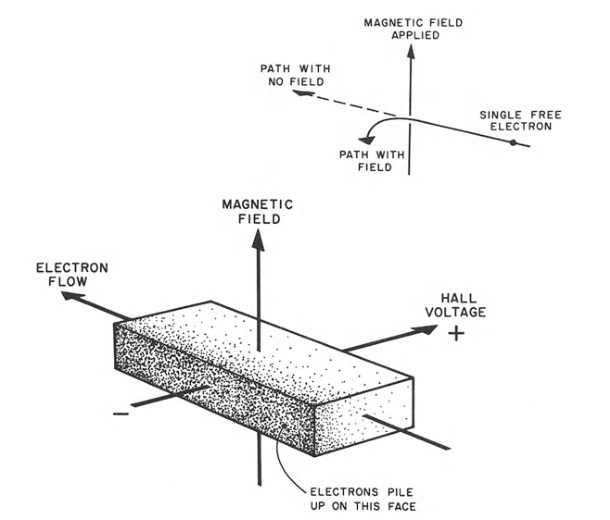
\includegraphics[width=\columnwidth]{hall-effect-hurd.png}
    \caption{A more "self-explanatory" diagram of the Hall effect}
\end{figure}

\subsection{Mechanism of OHE}

In the given figure, an electric current is passed along the $ x $ direction with corresponding current density is $ j_x $. The cause of this current is an external electric field along the same direction, $ E_x $.

An external magnetic field $ H $ along the $ z $ direction is applied and the Hall effect is observed.

From the Lorentz force equation

\begin{equation} \label{lorentz} 
    \vec{F} = q (\vec{E} + \vec{v} \times \vec{H})
\end{equation}

The second term of the \cref{lorentz} is responsible for deflecting the trajectory of the electrons in the negative $ y $-direction and accumulating along the sides of the material. As this accumulation takes place, an electric field builds up along the $ y $-direction which opposes the further deflection of electrons towards the sides. This process continues until an equilibrium is reached, at which this transverse field (or \textbf{Hall field}) $ E_y $ perfectly balances the Lorentz force and the current flows only along the longitudinal direction.

\subsection{Hall coefficient}

This transverse Hall field $ E_y $ can be thought of to be proportional to the external magnetic field $ H $ and longitudinal current density $ j_x $. Here, we define the Hall coefficient as

\begin{equation} \label{hall-coeff} 
    R_H = \frac{E_y}{j_x H} 
\end{equation}

A rather interesting point to note is that by our construction, $ j_x $ and $ H $ are along positive $ x $ and $ z $ directions respectively. $ E_y $ however, is along negative $ y $ direction, meaning that the resultant sign of the Hall coefficient $ R_H $ is negative.

Now, imagine if the charge carriers were positive, this would result in their velocity along $ x $-direction to get reversed ($ j_x $ would still be along positive $ x $-direction). The Lorentz force would remain unchanged (as can be seen from \cref{lorentz}). Consequentially, the direction of Hall field would be in the opposite direction compared to its direction in the case of negatively charged carriers. This would mean that measuring the Hall coefficient of a material, would help one determine the sign of the charge carriers.

\subsubsection{Calculating the Hall coefficient}

Let us consider current densities $ j_x $ and $ j_y $ in the presence of an electric field with components $ E_x $ and $ E_y $, and in the presence of an external magnetic field $ H $ along the $ z $-axis. 

The average force per electron is given by the Lorentz force equation, i.e. $ \vec{F} = -e (\vec{E} + \vec{v} \times \vec{H}) $, and hence the average momentum per electron becomes

\begin{equation}
    \frac{d \vec{p}}{dt} = -e \left( \vec{E} + \frac{\vec{p}}{m} \times H \right) - \frac{\vec{p}}{\tau} 
\end{equation}

During equilibrium, the current becomes time-independent, and hence $ p_x $ and $ p_y $ satisfy the equations

\begin{equation}
    \begin{split}
        0 &= -e E_x - \omega_c p_y - \frac{p_x}{\tau}\\
        0 &= -e E_y + \omega_c p_x - \frac{p_y}{\tau} 
    \end{split}
\end{equation}

where 

\begin{equation}
    \omega_c = \frac{e H}{m} 
\end{equation}

Solving the above equations, we get

\begin{equation}
    E_y = - \left( \frac{\omega_c \tau}{\sigma_0}  \right) j_x = - \left( \frac{H}{ne} \right) j_x
\end{equation}

This yields the Hall coefficient (\cref{hall-coeff}) to be

\begin{equation}
    R_H = - \frac{1}{ne}
\end{equation}

where $ n $ is the number density of the charge carriers.

This is a rather astonishing result, suggesting that the Hall coefficient of a material, depends solely on the density of the carriers.

We shall stop our investigation of the Ordinary Hall effect in lieu of the main topic of the report.

\section{Anomalous Hall effect}

The previous section dealt with OHE where the nature of the current carrying material is immaterial. Now, we deal with specific characteristics of such material, namely, magnetic metals.

It is observed that when observing Hall effect in such magnetic materials, certain unusual results are observed.
